\documentclass[../5RO17_TP4.tex]{subfiles}

\begin{document}
\section{Translation et Rotation}
\noindent Lorsqu'on manipule des nuages des points, différentes opérations deviennent necéssaires pour en faciliter la compréhension et, parfois, l'exploitation. Les principales transformations incluent la \textbf{translation} et \textbf{rotation}, qui ajustent la position et l'orientation des pointts dans l'espace tridimensionnel.


\subsection{Translation}
\noindent Pour réaliser une translation, chaque point du nuage de points est décalé en ajoutant une valeur fixe aux coordonnées $x$, $y$, et $z$ de chaque point. Cela permet de déplacer l’ensemble des points dans une direction spécifique tout en conservant leur structure relative. La translation peut être représentée comme suit:
\begin{equation}
    \begin{cases}
        x' = x + t_x\\
        y' = y + t_y\\
        z' = z + t_z\\
    \end{cases}
\end{equation}
\noindent Où $t_x$, $t_y$, et $t_z$ sont les valeurs de décalage appliquées respectivement aux axes $x$, $y$, et $z$. Cette opération simple peut être implémentée efficacement, comme illustré ci-dessous:\\

\begin{scriptsize}\mycode
	\begin{lstlisting}[language=Python, caption=\texttt{translation()}]
translation = np.array([0, -0.1, +0.1]).reshape((3, 1))

show_cloud(
    original_cloud + translation,
    title=f'{cloud_name}_translation',
    save=save
)
	\end{lstlisting}
\end{scriptsize}
\noindent Ainsi, la translation a été appliqué sur le nuage des points \texttt{Bunny} comme montré ci-dessous:
\begin{figure}[H]
    \centering
    \begin{subfigure}[b]{0.475\textwidth}
        \centering
        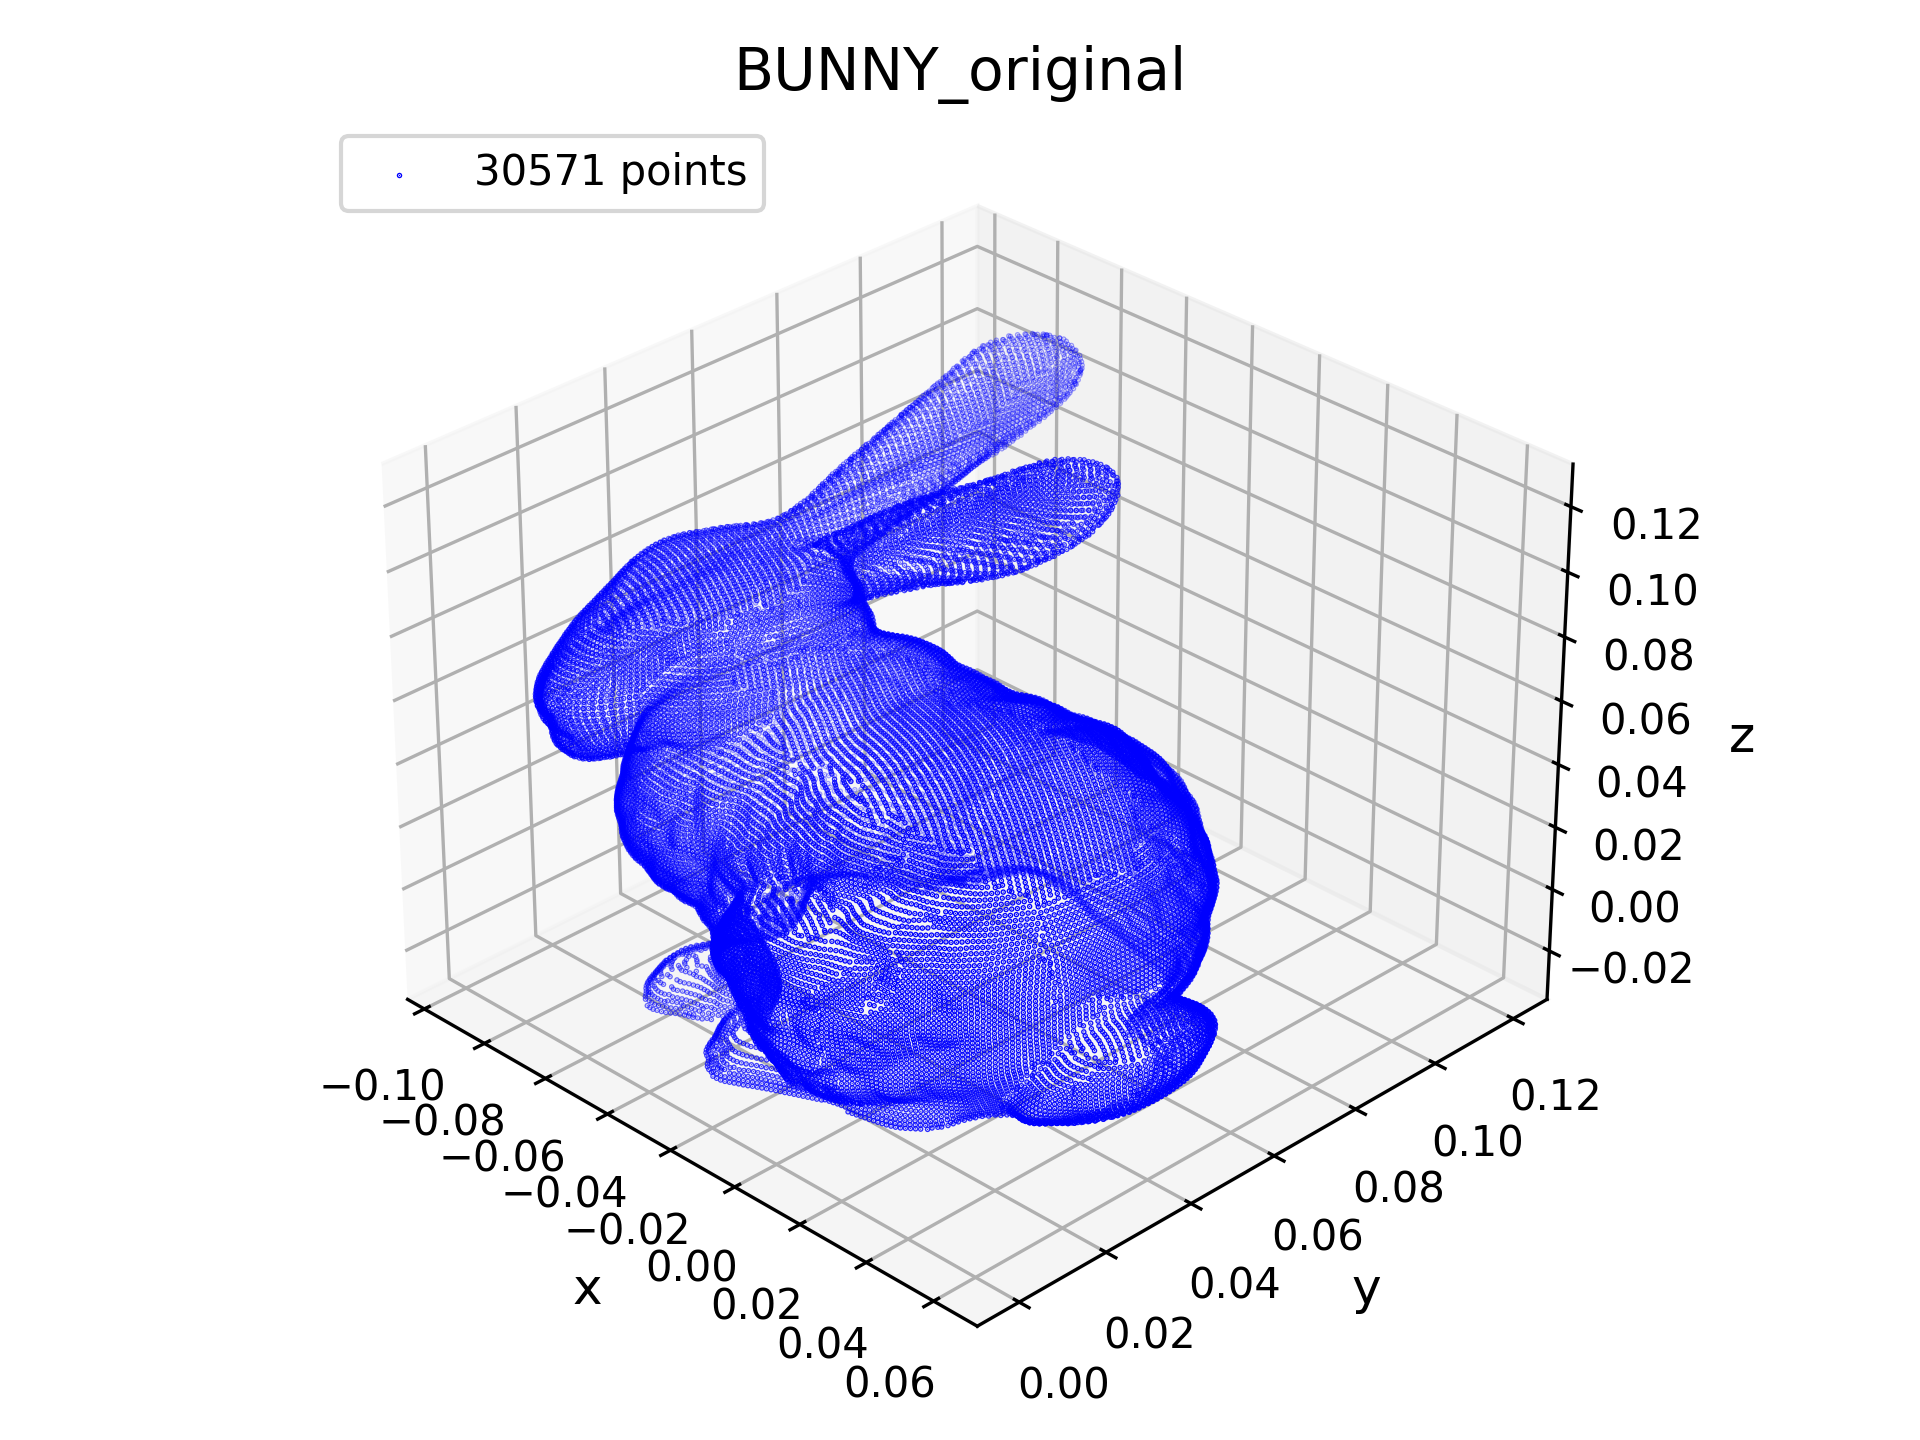
\includegraphics[width=\linewidth]{images/BUNNY_original.png}
        \caption{avant translation}
        \label{}
    \end{subfigure}\hfill
    \begin{subfigure}[b]{0.475\textwidth}
        \centering
        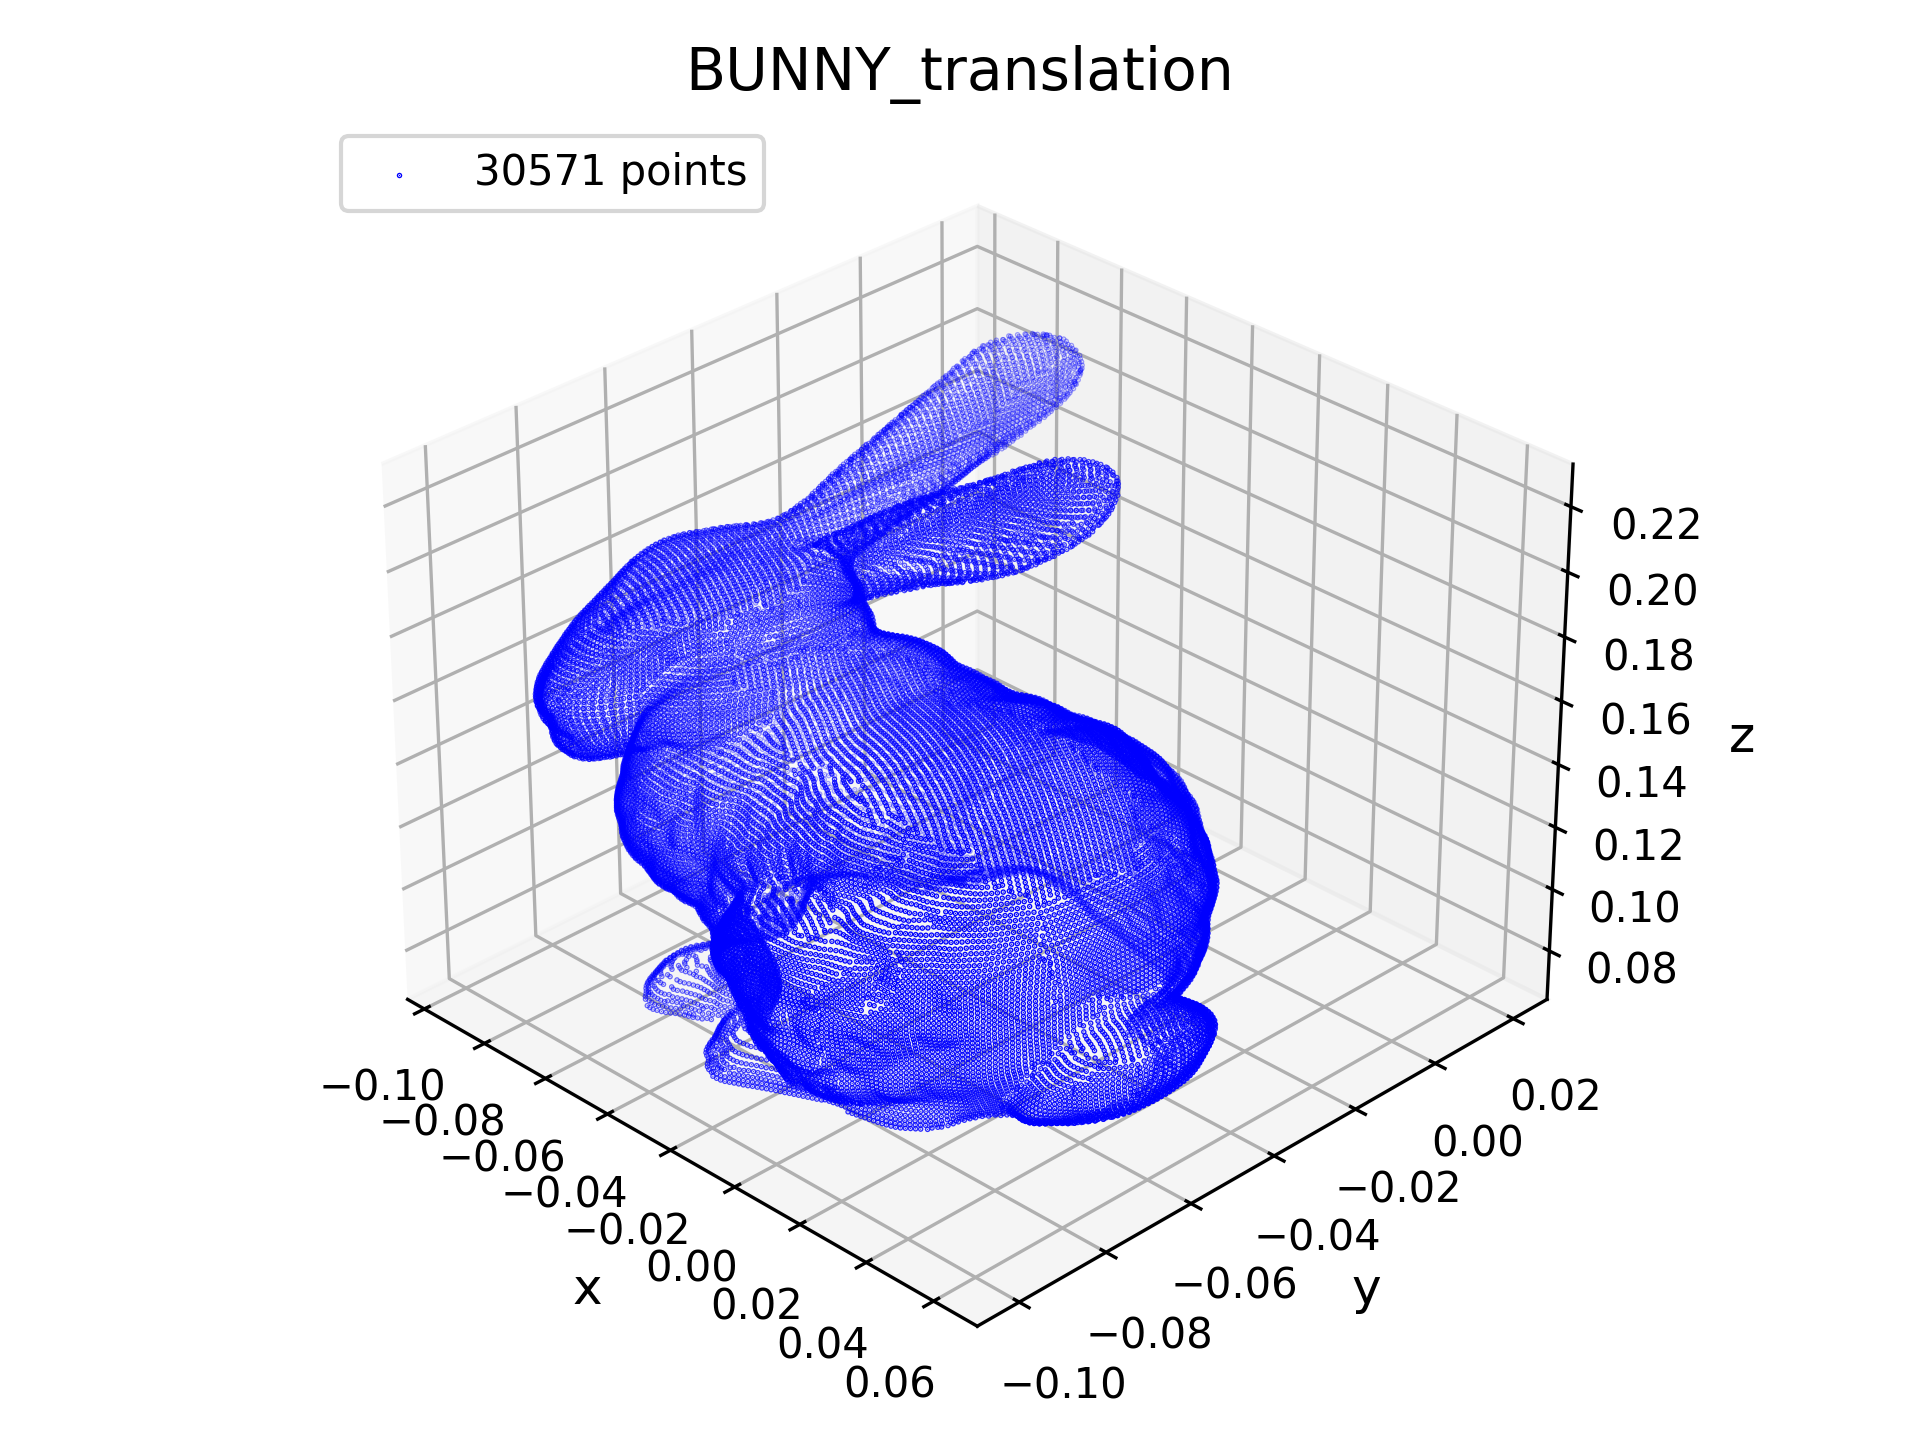
\includegraphics[width=\linewidth]{images/BUNNY_translation.png}
        \caption{après translation}
        \label{}
    \end{subfigure}
    \caption{Translation pour \texttt{Bunny}}
    \label{fig:translation}
\end{figure}
\begin{remark}
    Notons que seules les coordonnées de chaque point changent lors de la transformation, car la perspective globale du nuage de points demeure inchangée.\\
    
    \noindent En effet, cette transformation conserve les distances relatives entre les points, modifiant simplement leur orientation sans altérer la structure ou la forme du nuage.
\end{remark}


\subsection{Centralisation}
\noindent Pour réaliser une centralisation, on effectue une translation en fonction du centroïde, qui correspond à la moyenne des positions des points sur les axes $x$, $y$, et $z$. Cette opération ramène le nuage au centre de l'espace de référence en le décalant de manière à ce que le centroïde soit à l'origine, comme illustré ci-dessous:
\begin{equation}
    x' = x - \bar{x}
    \qquad
    y' = y - \bar{y}
    \qquad
    z' = z - \bar{z}
\end{equation}
\noindent Où $\bar{x}$, $\bar{y}$, et $\bar{z}$ sont les coordonnées moyennes respectives du nuage de points. Cette opération simple peut être implémentée efficacement, comme illustré ci-dessous:\\

\begin{scriptsize}\mycode
	\begin{lstlisting}[language=Python, caption=\texttt{centroid()}]
centroid = np.mean(original_cloud, axis=1).reshape((3, 1))
show_cloud(
    original_cloud - centroid
    title=f'{cloud_name}_centroid',
    save=save
)
	\end{lstlisting}
\end{scriptsize}
\noindent Ainsi, la centralisation a été appliqué sur le nuage des points \texttt{Bunny} comme montré ci-dessous:
\begin{figure}[H]
    \centering
    \begin{subfigure}[b]{0.475\textwidth}
        \centering
        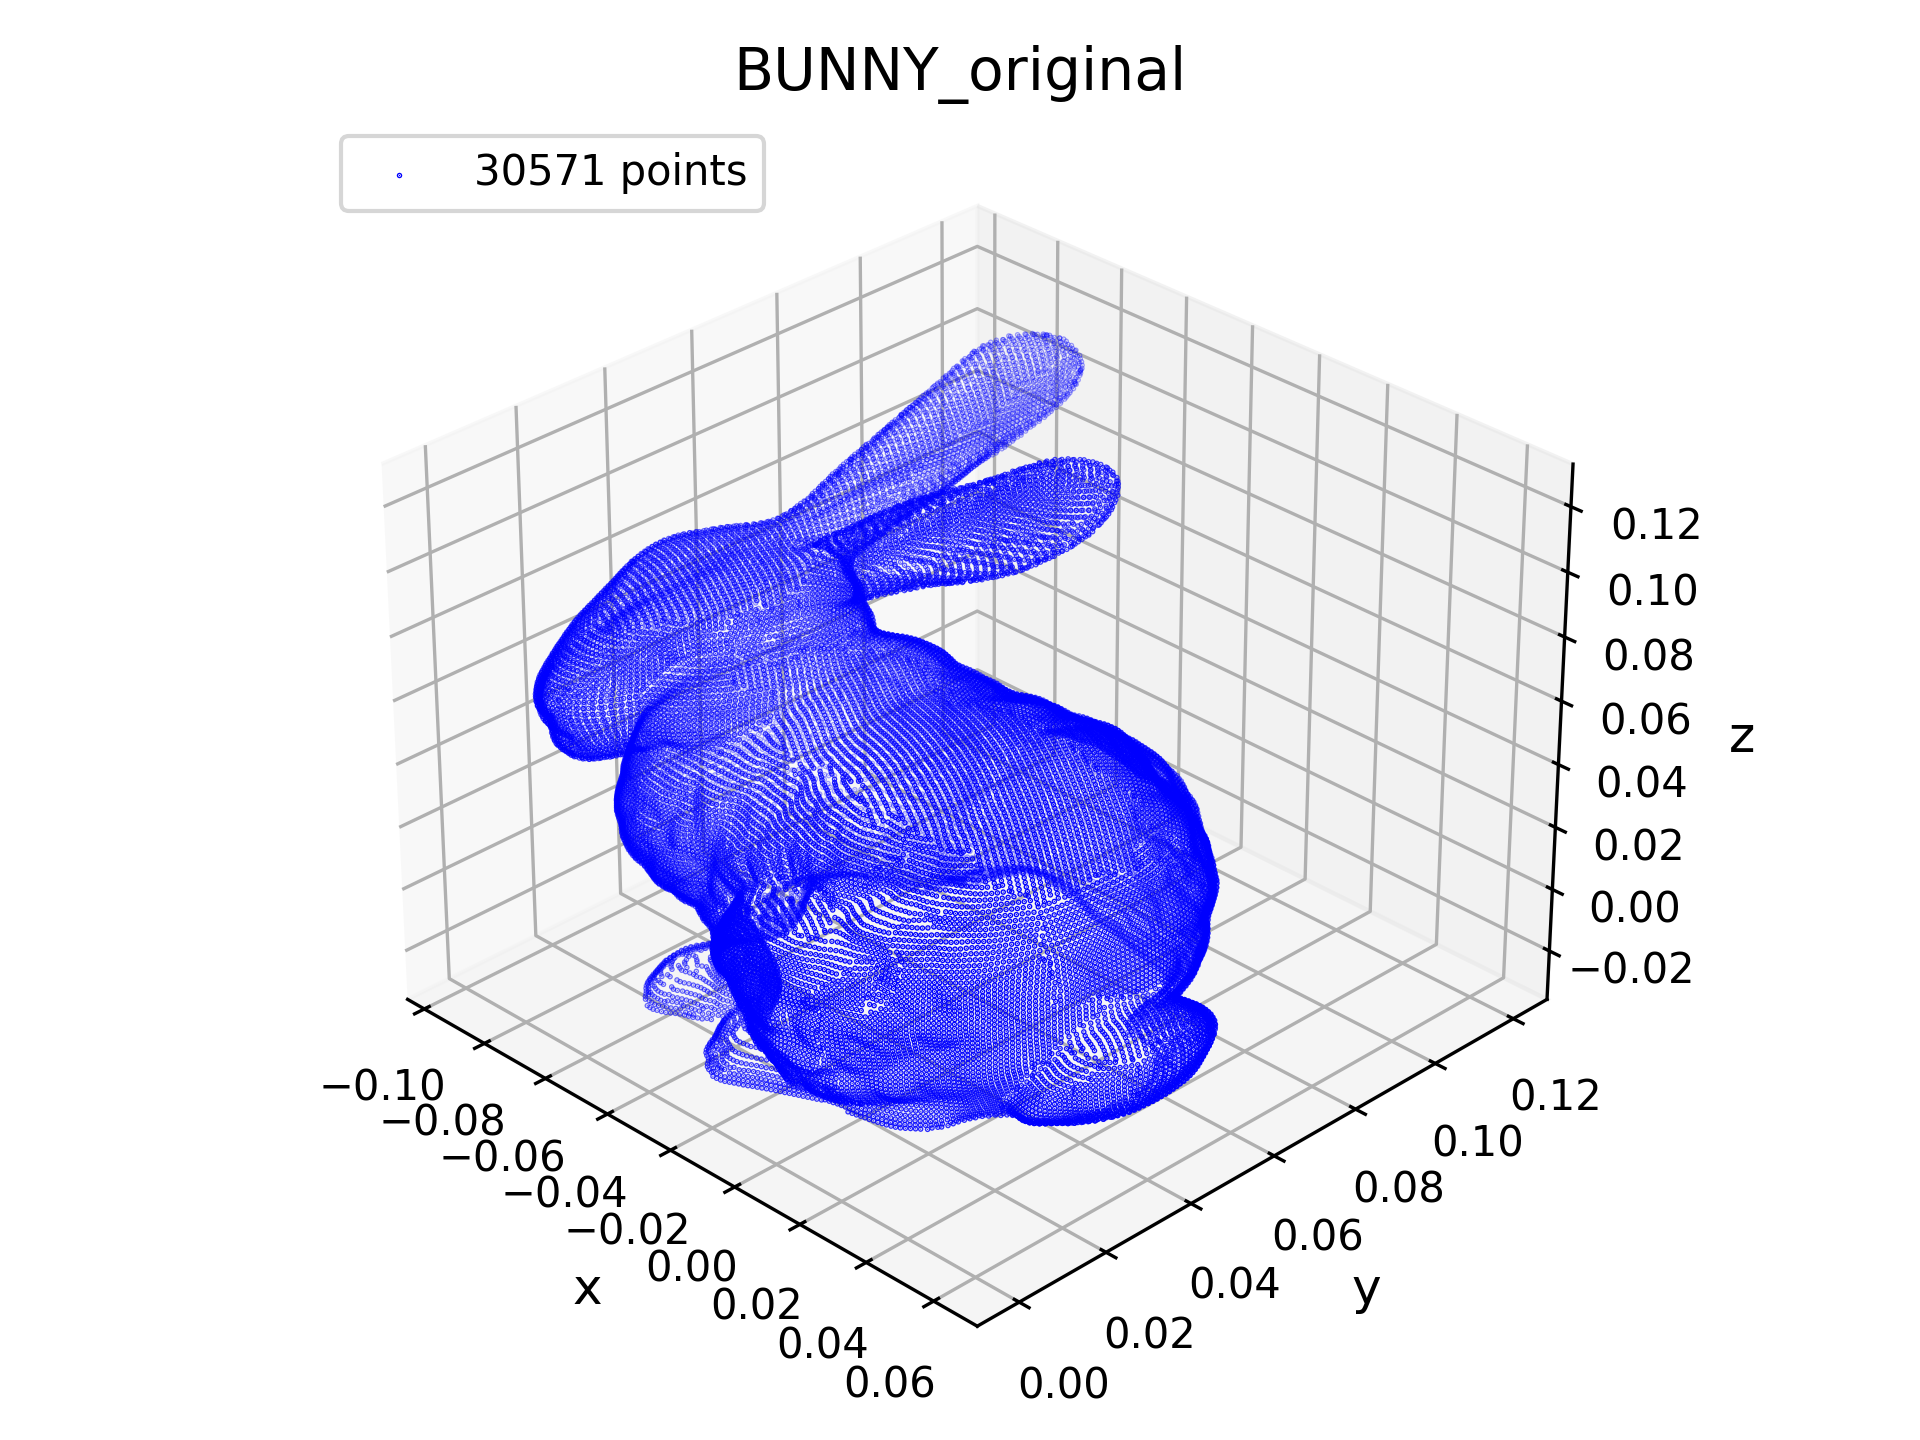
\includegraphics[width=\linewidth]{images/BUNNY_original.png}
        \caption{avant centralisation}
        \label{}
    \end{subfigure}\hfill
    \begin{subfigure}[b]{0.475\textwidth}
        \centering
        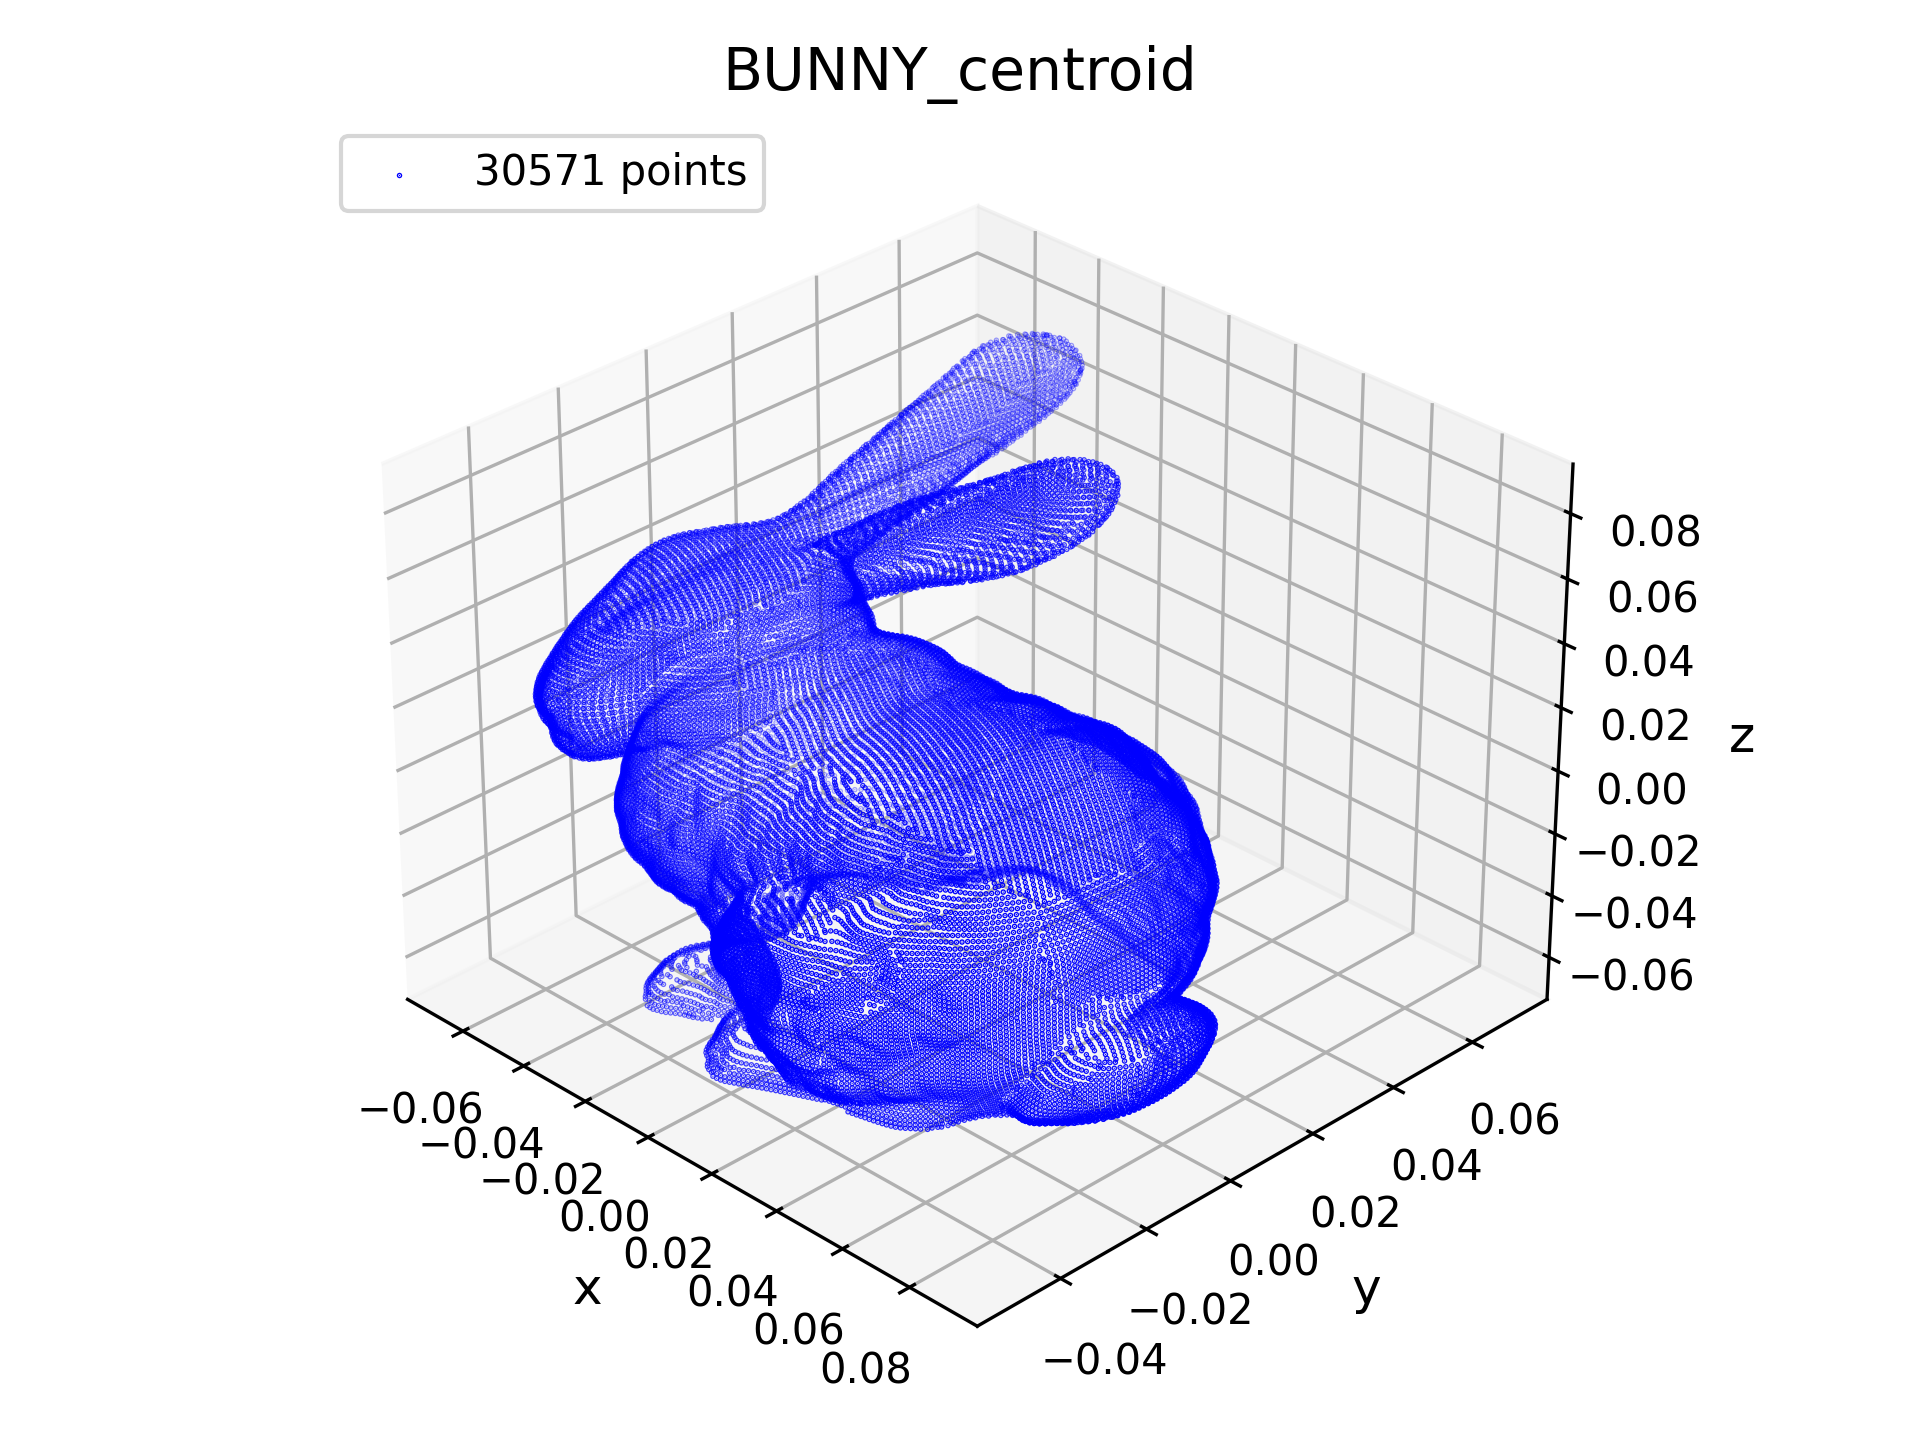
\includegraphics[width=\linewidth]{images/BUNNY_centroid.png}
        \caption{après centralisation}
        \label{}
    \end{subfigure}
    \caption{Centralisaion pour \texttt{Bunny}}
    \label{}
\end{figure}

\subsection{Changement d'échelle}
\noindent Pour effectuer un changement d’échelle, on multiplie ou divise chaque coordonnée des points du nuage par un facteur d’échelle $s$, ce qui modifie la taille du nuage de points tout en conservant ses proportions. Ce redimensionnement est illustré comme suit:
\begin{equation}
    x' = x \cdot s
    \qquad
    y' = y \cdot s
    \qquad
    z' = z \cdot s
\end{equation}
\noindent Où $s>1$ agrandit le nuage et $0<s<1$ le réduit. Cette opération simple peut être implémentée efficacement, comme illustré ci-dessous:\\
\begin{scriptsize}\mycode
	\begin{lstlisting}[language=Python, caption=\texttt{rescale()}]
scale = 2
show_cloud(
    original_cloud * scale
    title=f'{cloud_name}_rescale',
    save=save
)
	\end{lstlisting}
\end{scriptsize}
\noindent Ainsi, le changement d'échelle a été appliqué sur le nuage des points \texttt{Bunny} comme montré ci-dessous:
\begin{figure}[H]
    \centering
    \begin{subfigure}[b]{0.475\textwidth}
        \centering
        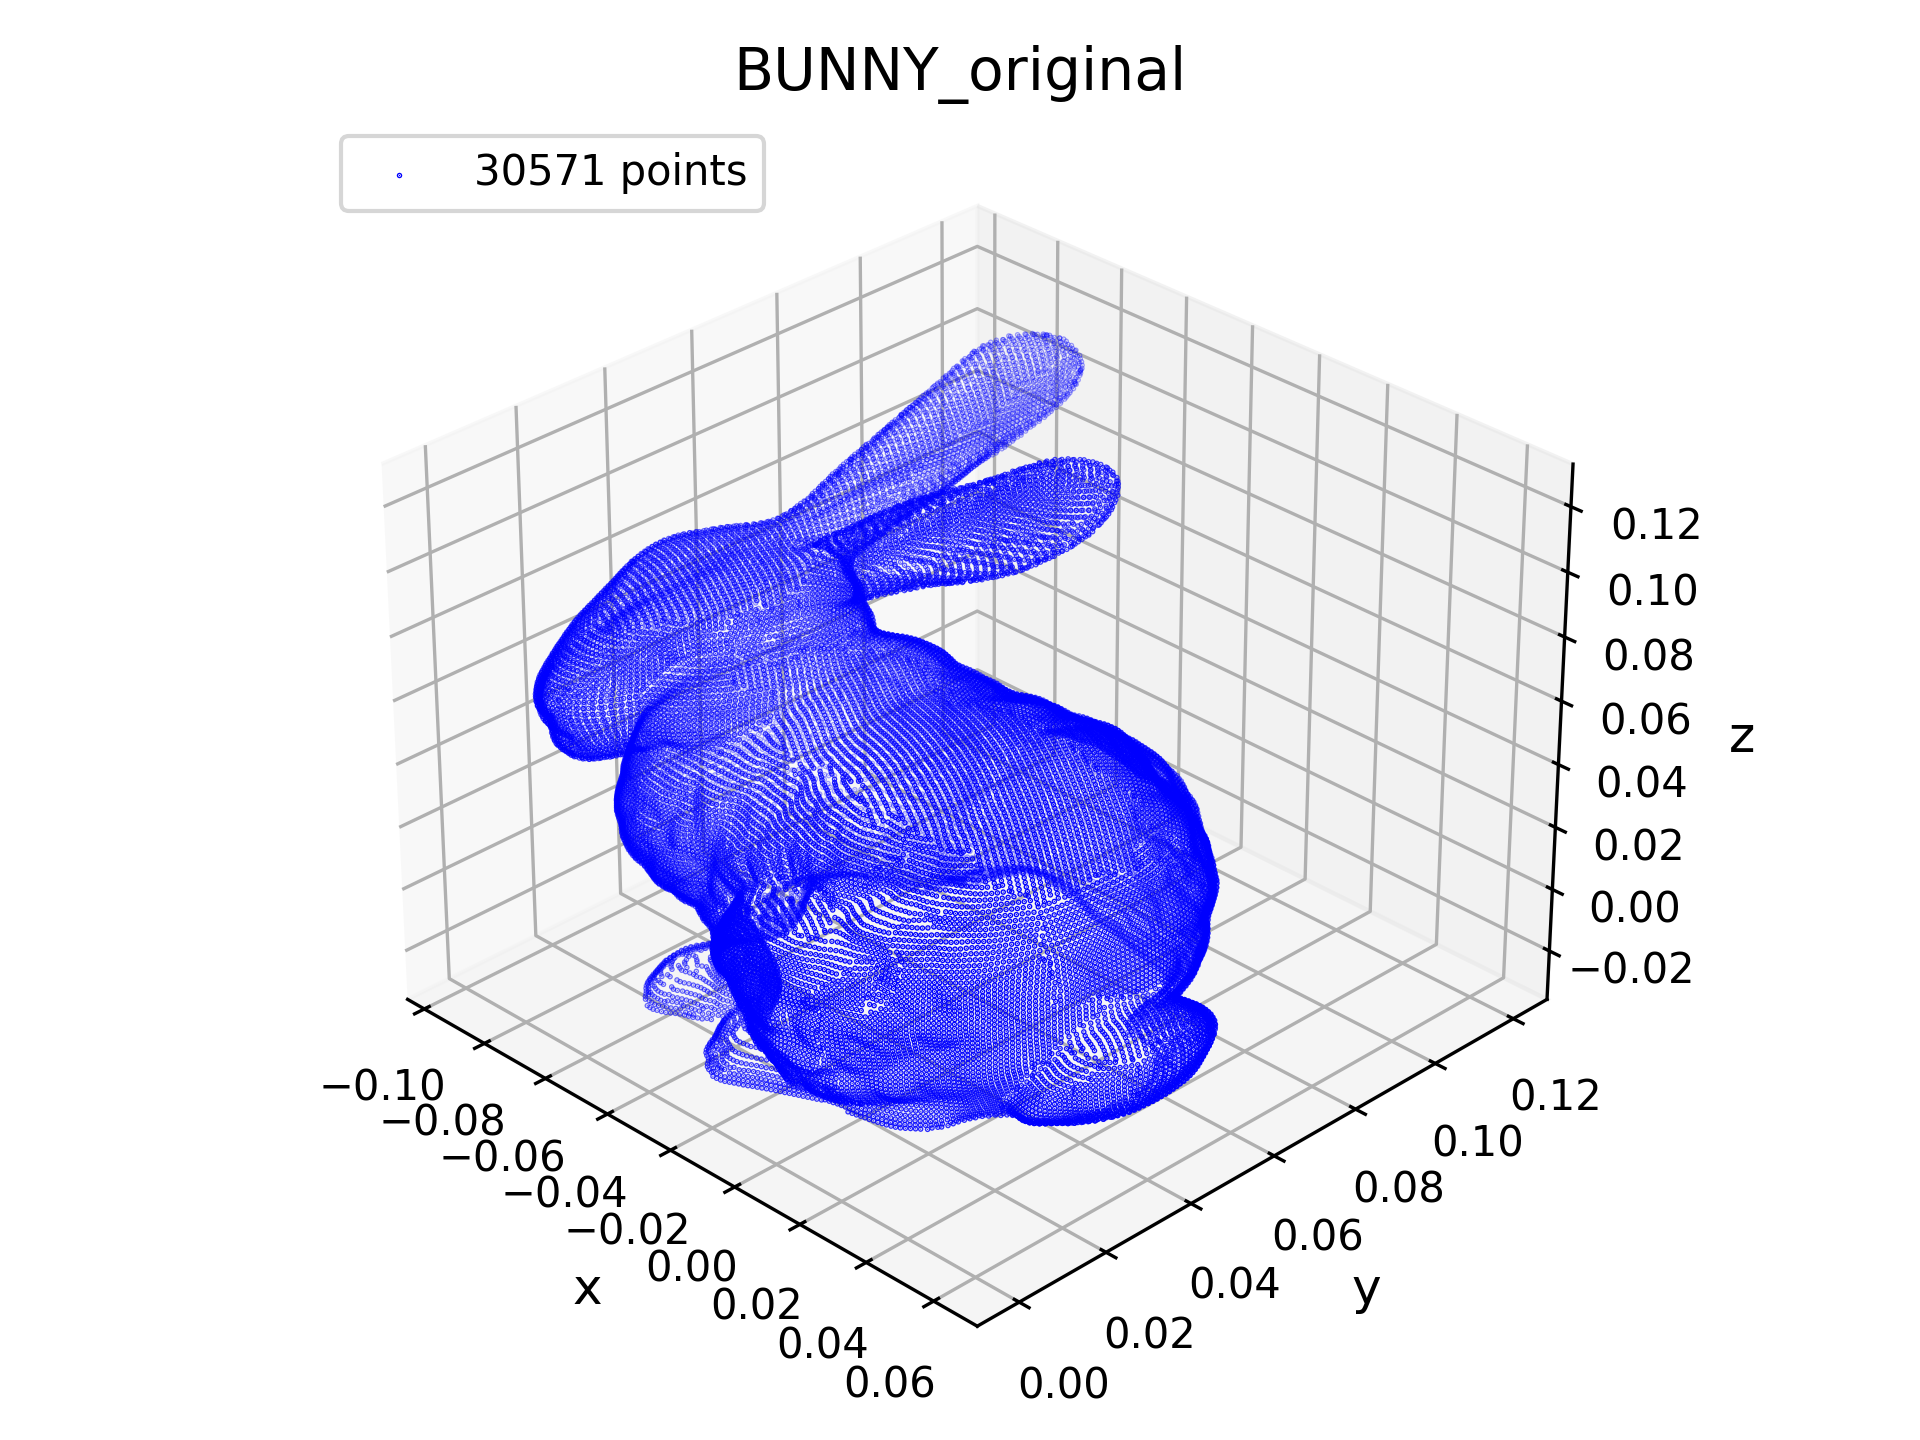
\includegraphics[width=\linewidth]{images/BUNNY_original.png}
        \caption{avant changement d'échelle}
        \label{}
    \end{subfigure}\hfill
    \begin{subfigure}[b]{0.475\textwidth}
        \centering
        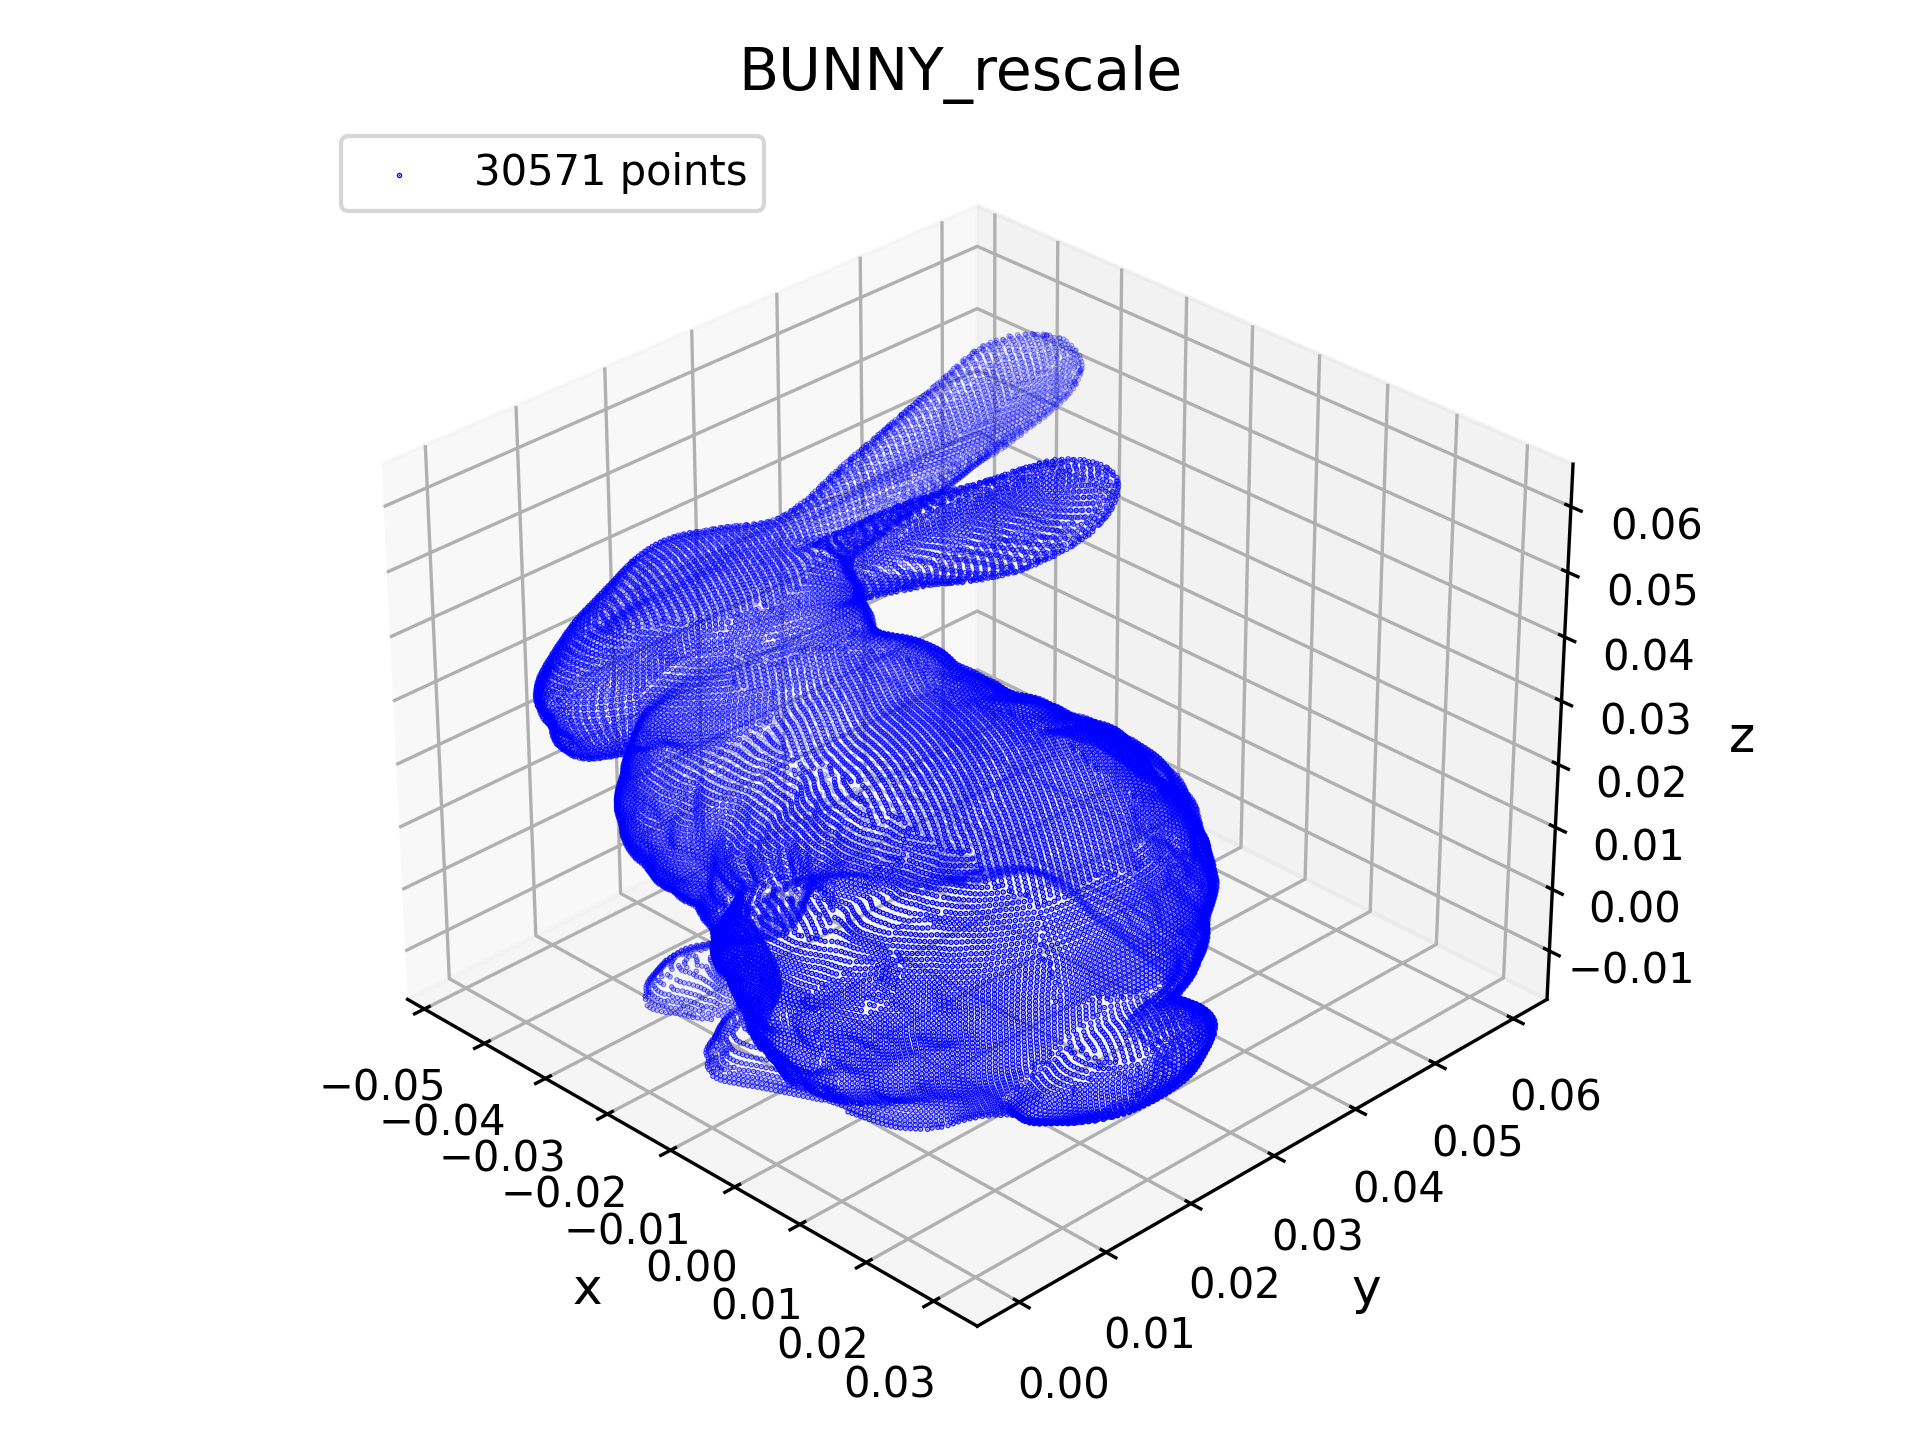
\includegraphics[width=\linewidth]{images/BUNNY_rescale.png}
        \caption{après changement d'échelle}
        \label{}
    \end{subfigure}
    \caption{Changement d'échelle pour \texttt{Bunny}}
    \label{}
\end{figure}

\subsection{Rotation}
\noindent Pour effectuer une rotation autour de l'axe $z$, chaque point du nuage est multiplié par une matrice de rotation $R(\theta)$, définie par l'angle de rotation $\theta$. Cette opération conserve les distances et modifie seulement l’orientation du nuage autour de l’axe choisi. La matrice $R(\theta)$ est donnée par:
\begin{equation}
    (x', y', z') = R(\theta) \cdot (x, y, z)
    \qquad
    \text{où}
    \quad
    R_z(\theta) = 
    \begin{bmatrix}
        \cos \theta & -\sin \theta & 0 \\
        \sin \theta & +\cos \theta & 0 \\
        0 & 0 & 1 \\
    \end{bmatrix}
\end{equation}
\noindent Cette opération simple peut être implémentée efficacement, comme illustré ci-dessous:\\
\begin{scriptsize}\mycode
	\begin{lstlisting}[language=Python, caption=\texttt{rotation()}]
theta = np.pi / 3
show_cloud(
    rotation_matrix(theta).dot(original_cloud),
    title=f'{cloud_name}_rotation_{theta}',
    save=save
)
	\end{lstlisting}
\end{scriptsize}
\noindent Ainsi, la rotation autour de $z$ de $\theta = \pi / 3$ a été appliqué sur le nuage des points \texttt{Bunny} comme montré ci-dessous:
\begin{figure}[H]
    \centering
    \begin{subfigure}[b]{0.475\textwidth}
        \centering
        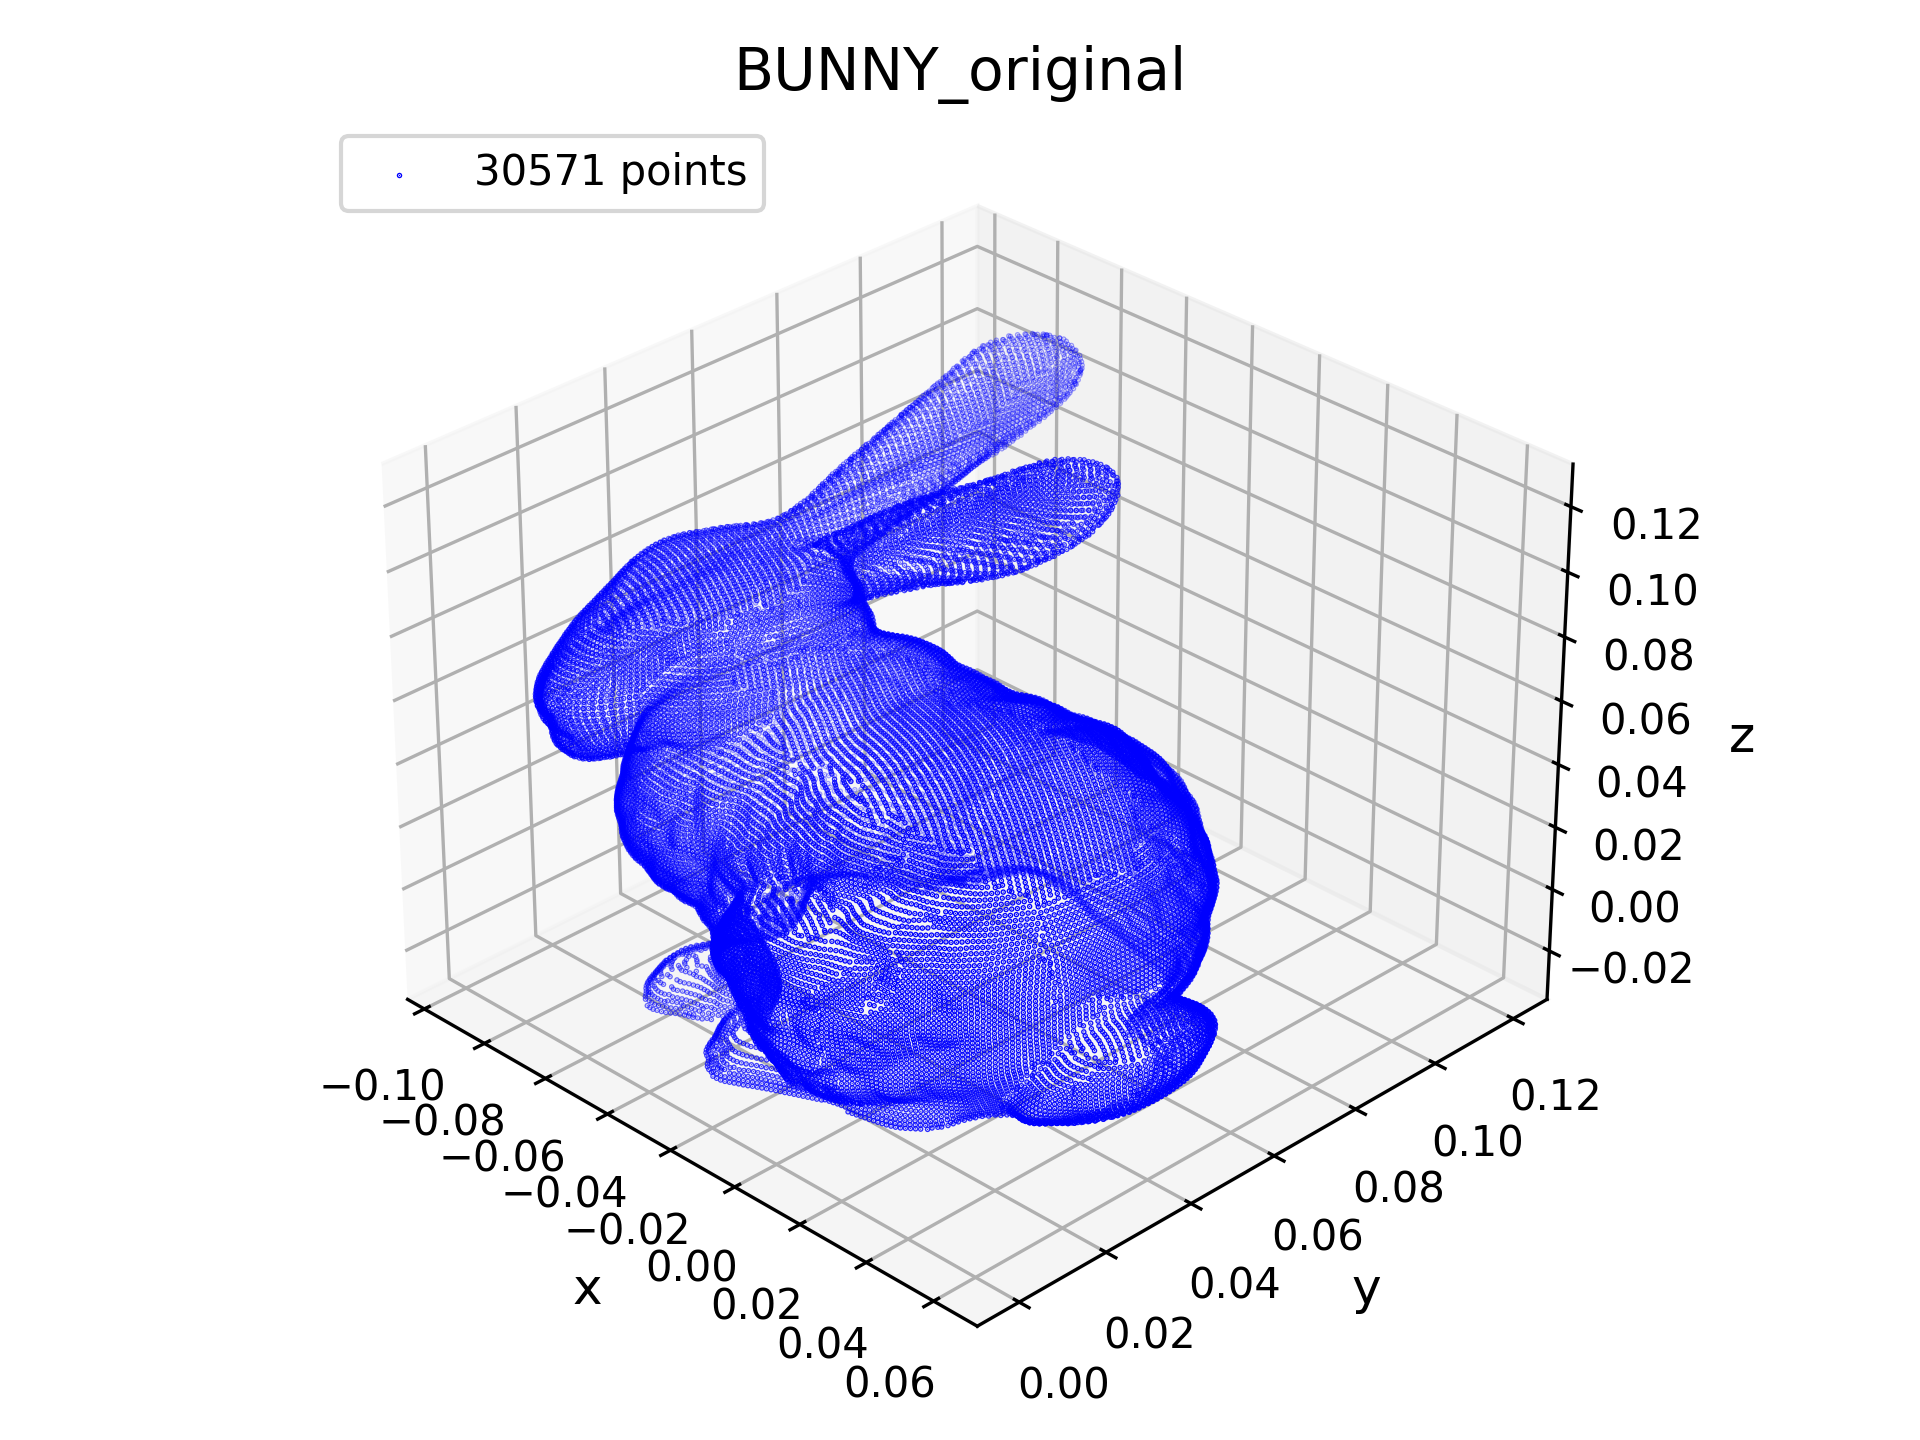
\includegraphics[width=\linewidth]{images/BUNNY_original.png}
        \caption{avant rotation}
        \label{}
    \end{subfigure}\hfill
    \begin{subfigure}[b]{0.475\textwidth}
        \centering
        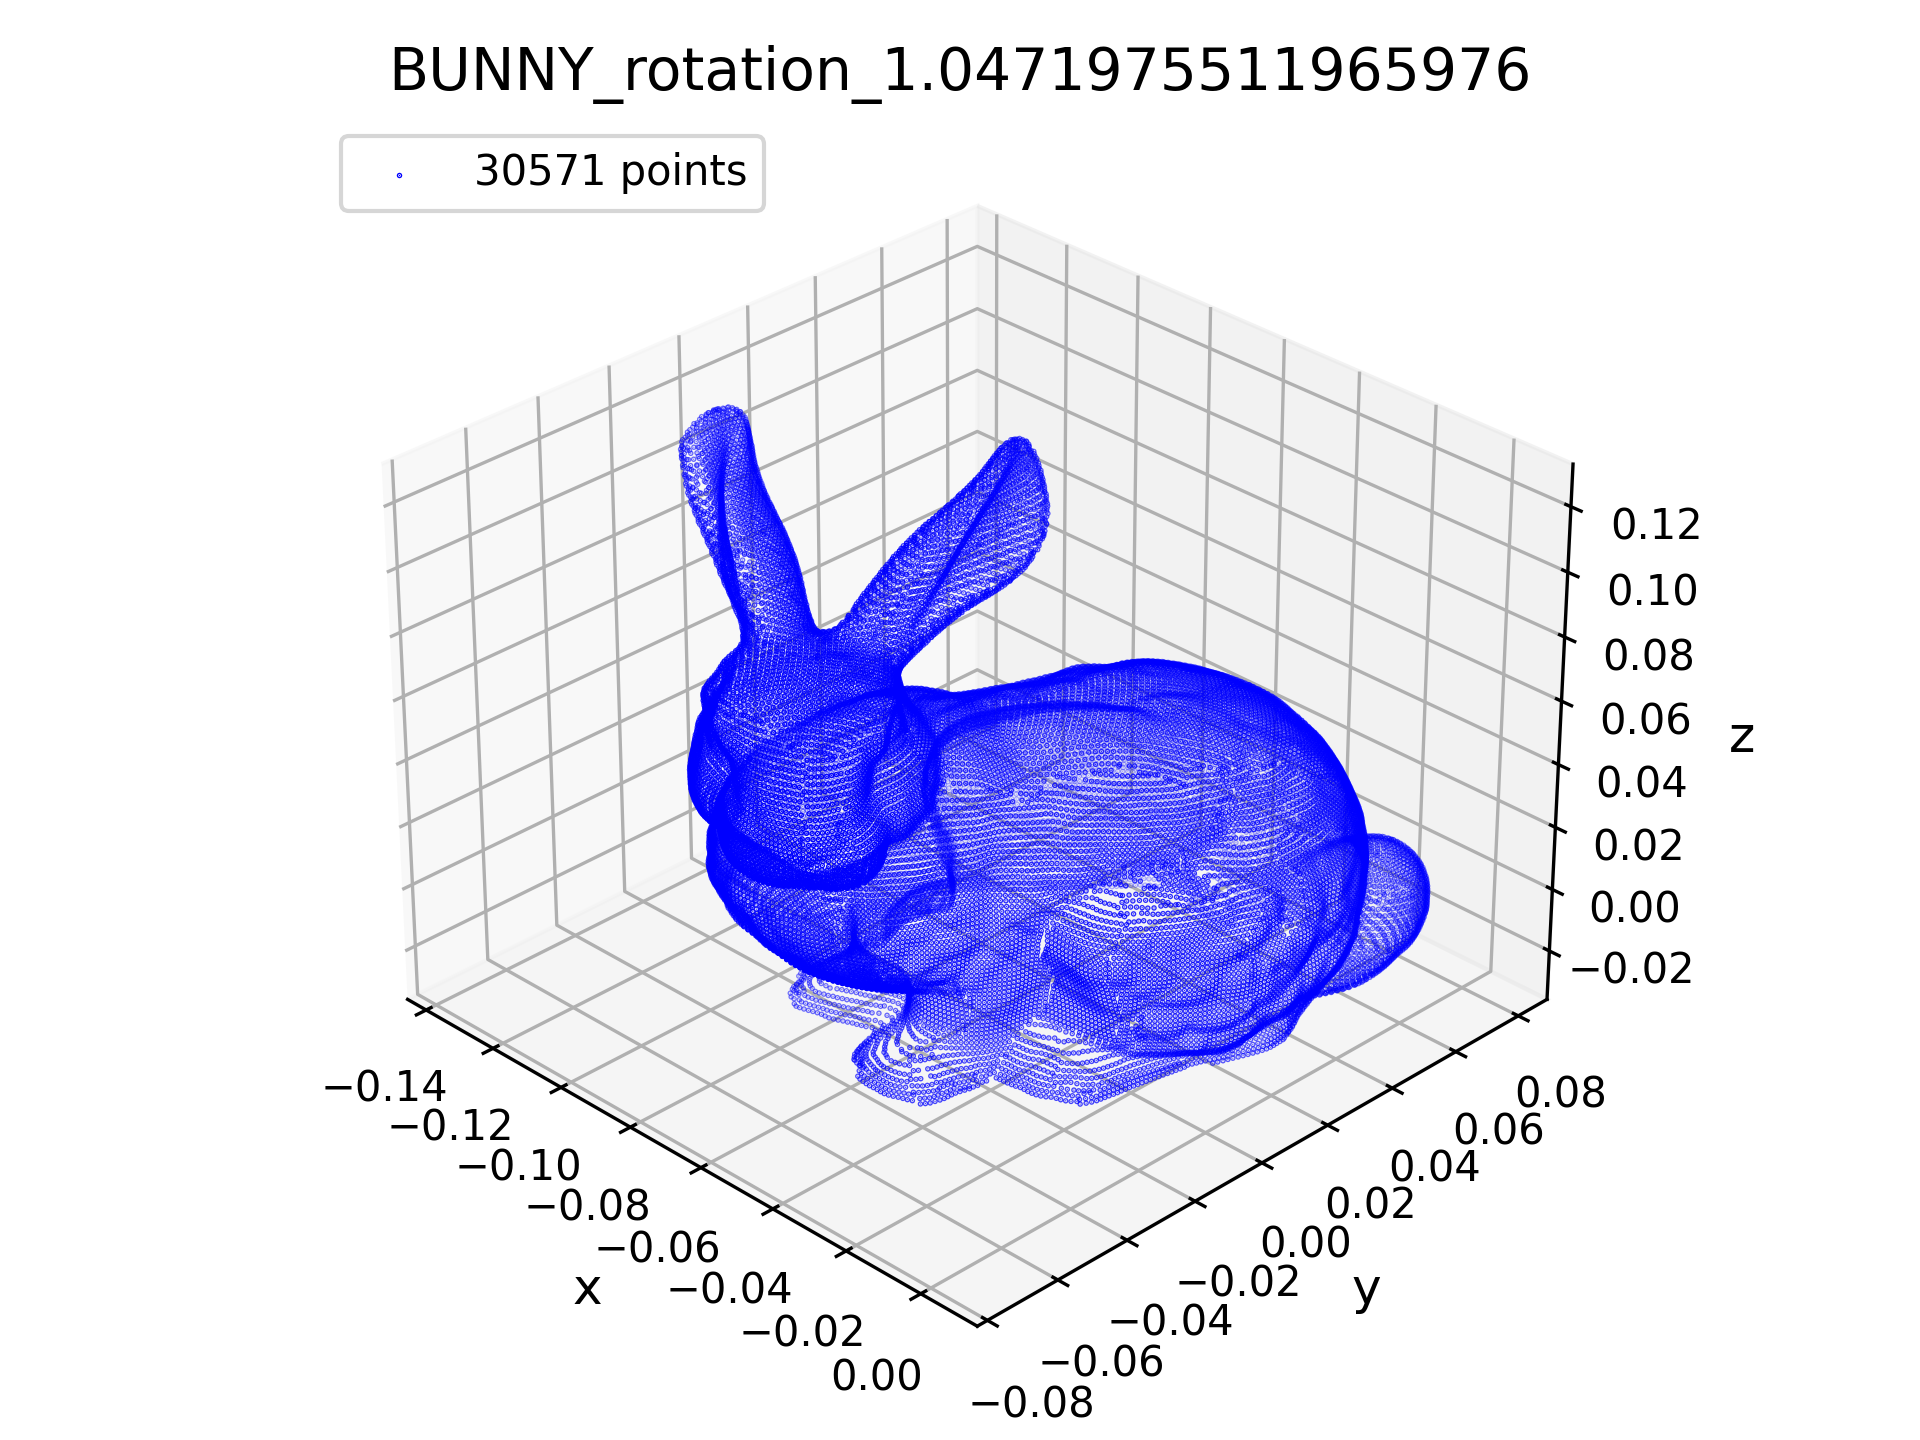
\includegraphics[width=\linewidth]{images/BUNNY_rotation_1.0471975511965976.png}
        \caption{après rotation}
        \label{}
    \end{subfigure}
    \caption{Rotation pour \texttt{Bunny}}
    \label{}
\end{figure}
\end{document}
